\section*{Задание}
\addcontentsline{toc}{section}{Задание}

Разработать программу "Виндоуз мобиле", функционирующую в рамках пяти процессов
(отец и 4 сына). Процесс-отец, имитируя работу ядра ОС, порождает 4
процесса-сына. Каждый сын регистрирует функцию-обработчик сигнала \texttt{SIGUSR1} и
переходит в состояние ожидания посредством pause(). Процесс-отец читает со
стандартного ввода цифру в диапазоне 0 \ldots ~3 (имитация касания какой-либо иконки
на экране планшета/смартфона) и посылает сигнал \texttt{SIGUSR1} соответствующему
процессу-сыну. Разбуженный сигналом процесс считывает со стандартного ввода одну
строку символов, преобразует её соответственно своей функциональности, выводит
результат в стандартный вывод и возвращается в состояние сна. Процессы-сыновья
имеют следующие функциональности:
\begin{itemize}
    \item 0 - смена "регистра" всех символов;
    \item 1 - инвертирование строки - первый символ становится последним и т.д.;
    \item 2 - обмен соседних символов - нечетный становится на место четного и наоборот;
    \item 3 - перевод в КОИ-8 - установление в 1 старшего (8-ого) бита каждого символа.
\end{itemize}
Для чтения цифры с клавиатуры в процессе-отце использовать неканонический режим.

\newpage

\section*{Описание структуры программы}
\addcontentsline{toc}{section}{Описание структуры программы}

В реализации данной программы было использовано 5 процессов: 1 родительский и 4 дочерних.
Родительский процесс считывает ввод пользователя, обрабатывает его и на его
основе запускает необходимый дочерний процесс, используя сигнал \texttt{SIGUSR1}.

Дочерний сигнал считывает строку символов, выполняет характерное действие над
ней и заного активирует родительский процесс.

Этот цикл повторяется, пока не будет нажата комбинация клавиш \^{}C, после чего
произойдет поочередное завершение всех дочерних процессов и выход из программы

Более подробная схема использования сигналов в программе приведена на рис. \ref{fig:signals}

\begin{figure}[h]
    \centering
    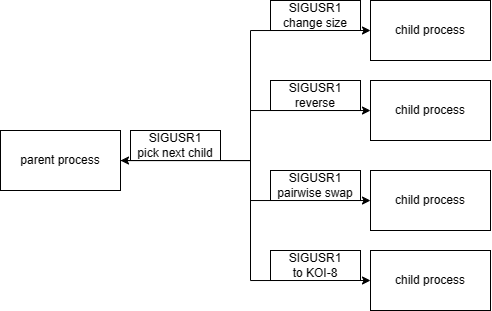
\includegraphics[width=0.75\linewidth]{images/lab1_signals.drawio.png}
    \caption{Схема распространения сигналов}
    \label{fig:signals}
\end{figure}

Для работы с терминалом используется неканонический режим ввода с сокрытием
вводимых символов. Таким образом достигается большая <<интерактивность>> всего
процесса пользования.

\newpage

\section*{Блок-схема программы}
\addcontentsline{toc}{section}{Блок-схема программы}

\begin{figure}[h]
    \centering
    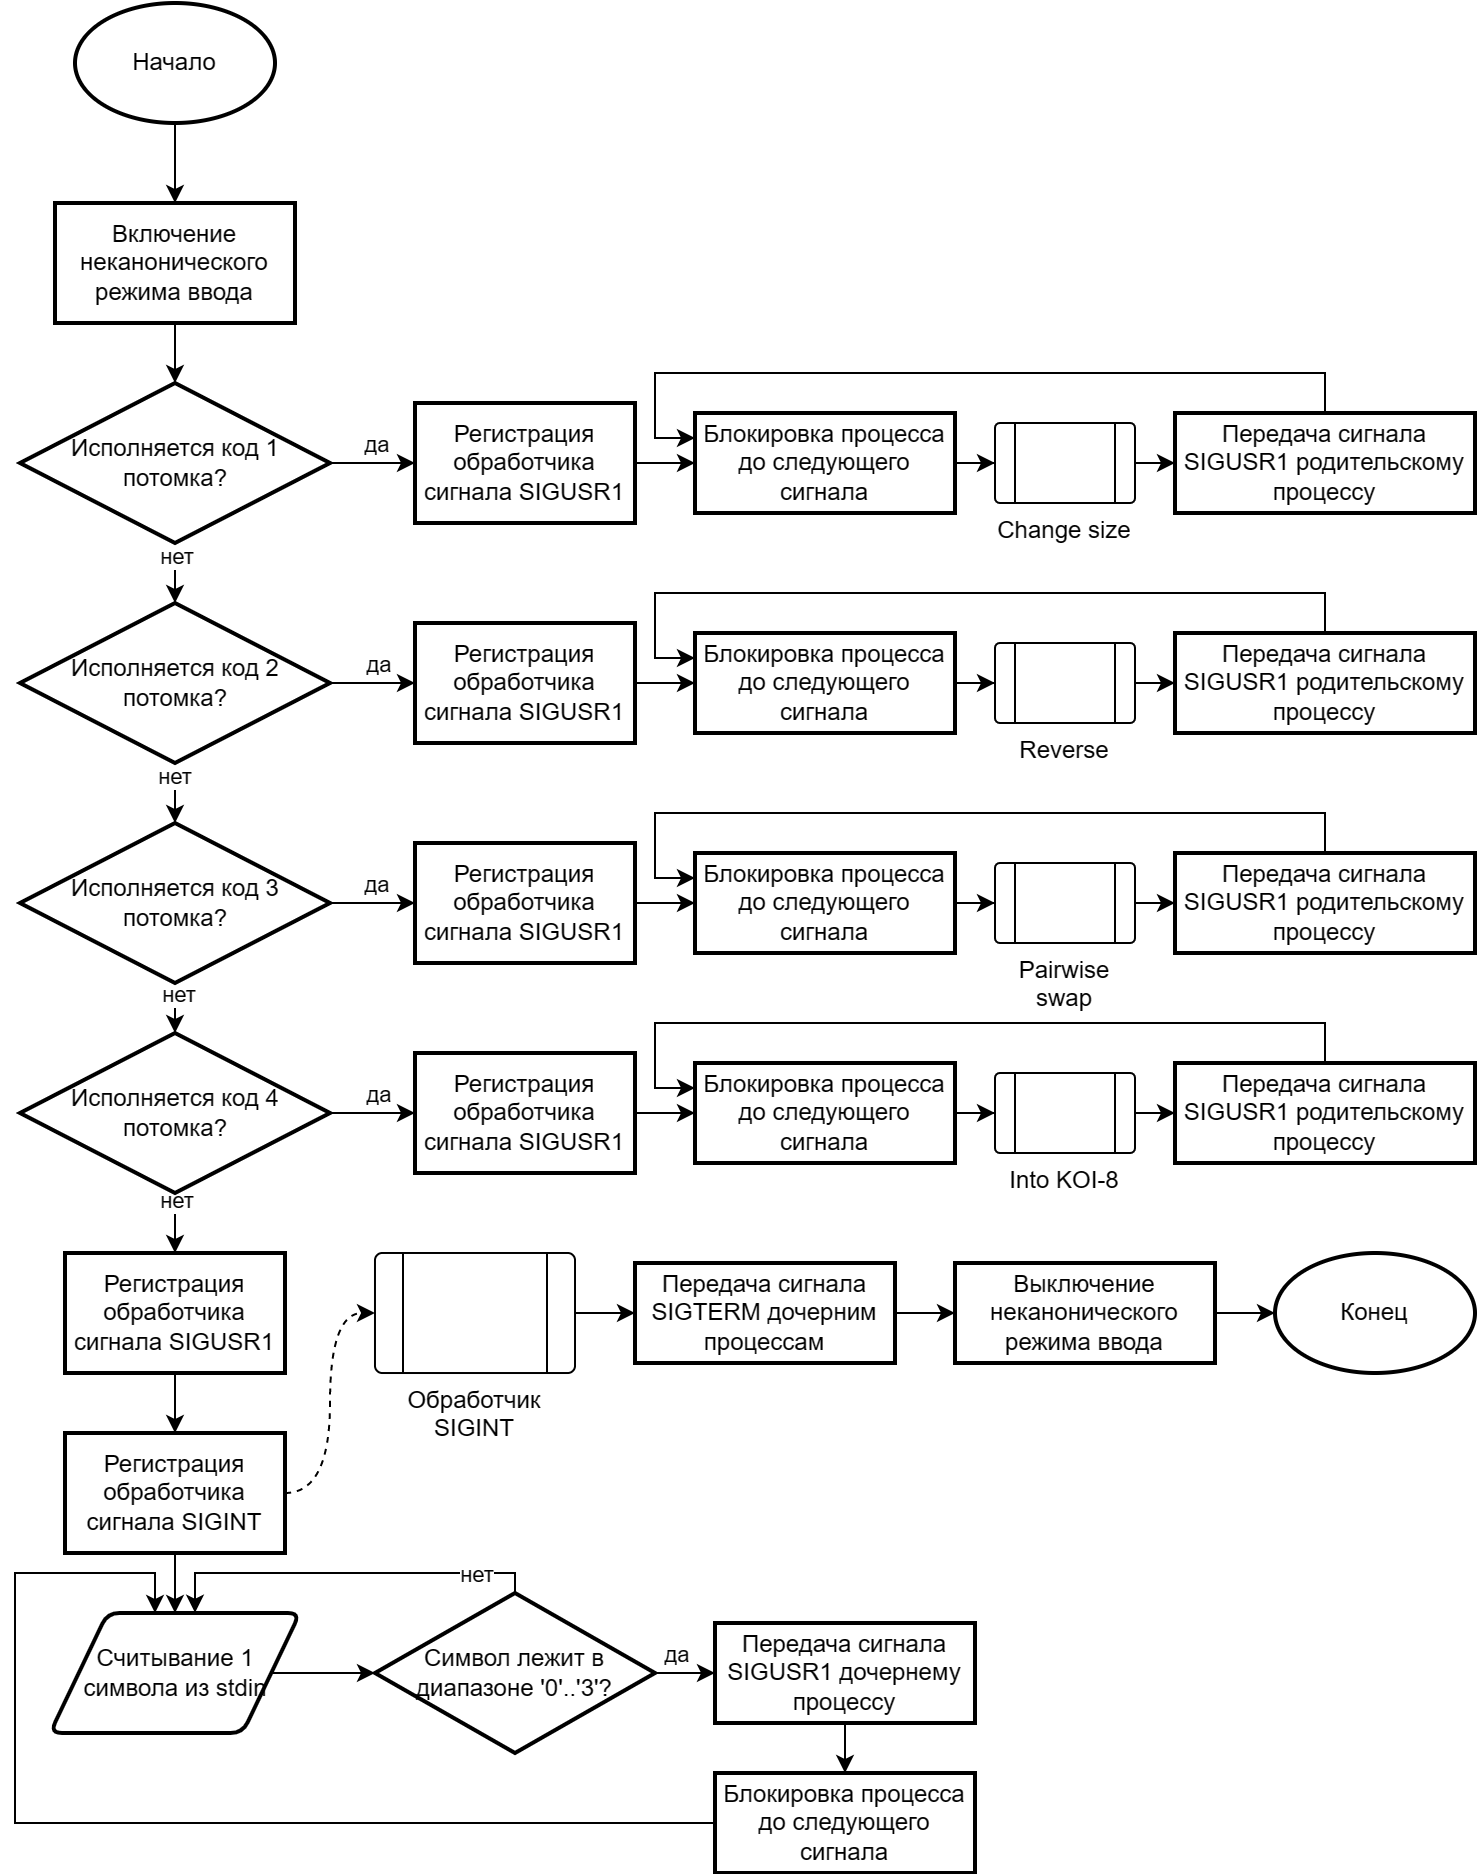
\includegraphics[width=0.75\linewidth]{images/lab1_block_scheme.drawio.png}
    \caption{Основная блок-схема программы}
    \label{fig:flowchart}
\end{figure}

\begin{figure}[h]
    \centering
    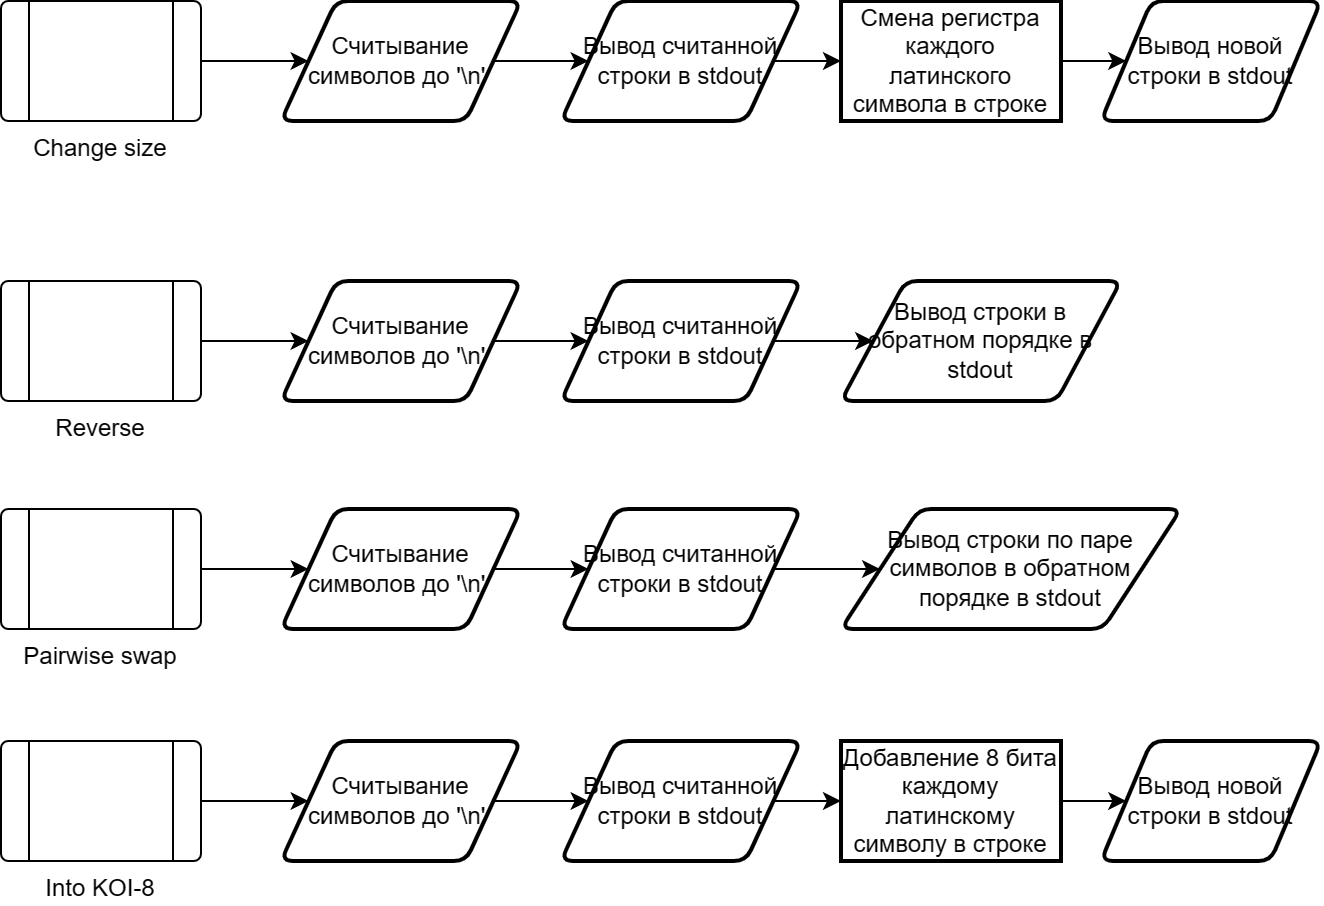
\includegraphics[width=0.75\linewidth]{images/lab1_invert_scheme.drawio.png}
    \caption{Блок-схема каждого подпроцесса программы}
    \label{fig:flowchart_other}
\end{figure}

\newpage

\section*{Результат работы}
\addcontentsline{toc}{section}{Результат работы}

Ниже показан результат работы при вводе в поток стандартного ввода следующей
последовательности: $0Hello\backslash n1Hello\backslash n2Hello\backslash n3Hello$

\begin{figure}[h]
    \centering
    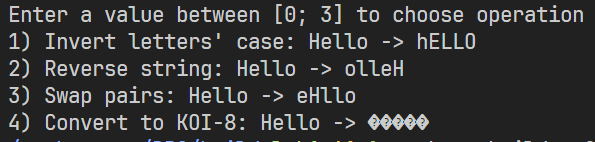
\includegraphics[width=0.75\linewidth]{images/lab1_output.png}
    \caption{Вывод программы в поток стандартного вывода}
    \label{fig:output}
\end{figure}

Примечание: в 4 случае вывод производился в консоль в режиме UTF8, поэтому там
присутствуют "битые" символы.

\newpage

\appendix

\section*{Приложение}
\section*{Текст программы}
\addcontentsline{toc}{section}{Текст программы}

\begin{verbatim}
include/handler.h:

#pragma once

/// Reads a string from [stdin], outputs it back to [stdout] and outputs the same string to [stdout] but latin letters
/// has inverted case
int invert_case();

/// Reads a string from [stdin], outputs it back to [stdout] and outputs it reversed variant to [stdout]
int reverse_str();

/// Reads a string from [stdin], outputs it back to [stdout] and outputs a string to [stdout] with original contents but
/// pairs of letters swapped with each other
int pairwise_swap();

/// Reads a string from [stdin], outputs it back to [stdout] and outputs a string to [stdout] where latin letters
/// converted to russian ones with inverted case
int convert_koi8();

src/handler.c:

#include <stdbool.h>
#include <stdio.h>
#include <stdlib.h>
#include <unistd.h>

#include "handler.h"
#include "utils.h"

/// Reads a string char-by-char to [buffer] from [stdin] and simultaneously outputs its contents.
/// Saves string's length to [size] pointer
static int read_line(char *buffer, size_t *size) {
    char c;
    size_t index = 0;

    while (true) {
        read(STDIN_FILENO, &c, 1);
        if (c == '\n')
            break;

        buffer[index++] = c;
        write(STDOUT_FILENO, &c, 1);
    }
    buffer[index] = '\0';
    *size = index;
    WRITE(STDOUT_FILENO, " -> ");

    return 0;
}

int invert_case() {
    WRITE(STDOUT_FILENO, "1) Invert letters' case: ");
    static char line[BUFSIZ];
    size_t size;

    if (read_line(line, &size) != 0)
        return 0;

    for (size_t i = 0; i < size; i++) {
        char c = line[i];

        if ('a' <= c && c <= 'z') {
            c = c - 'a' + 'A';
        } else if ('A' <= c && c <= 'Z') {
            c = c - 'A' + 'a';
        }

        write(STDOUT_FILENO, &c, 1);
    }

    return 0;
}

int reverse_str() {
    WRITE(STDOUT_FILENO, "2) Reverse string: ");
    static char line[BUFSIZ];
    size_t size;

    if (read_line(line, &size) != 0)
        return 0;

    for (size_t i = 0; i < size; i++)
        write(STDOUT_FILENO, &line[size - i - 1], 1);

    return 0;
}

int pairwise_swap() {
    WRITE(STDOUT_FILENO, "3) Swap pairs: ");
    static char line[BUFSIZ];
    size_t size;

    if (read_line(line, &size) != 0)
        return 0;

    for (size_t i = 0; i < size - 1; i += 2) {
        char pair[] = {line[i + 1], line[i]};
        write(STDOUT_FILENO, pair, 2);
    }

    if (size % 2 == 1)
        write(STDOUT_FILENO, &line[size - 1], 1);

    return 0;
}

int convert_koi8() {
    WRITE(STDOUT_FILENO, "4) Convert to KOI-8: ");
    static char line[BUFSIZ];
    size_t size;

    if (read_line(line, &size) != 0)
        return 0;

    for (size_t i = 0; i < size; i++) {
        char c = line[i];
        if (('a' <= c && c <= 'z') || ('A' <= c && c <= 'Z'))
            c |= 1 << 7;
        write(STDOUT_FILENO, &c, 1);
    }

    return 0;
}

include/utils.h:

#pragma once

#include <stdio.h>
#include <stdlib.h>

#if DEBUG
#define DEBUG_PRINT(file, format, ...) fprintf(file, format, __VA_ARGS__)
#else
#define DEBUG_PRINT(...) 0
#endif

/// Checks if pointer is not null, otherwise returns [default] value and prints debug message to stderr (in debug mode
/// only)
#define RETURN_DEFAULT_IF_NULL(ptr, default)                                                                           \
    if ((ptr) == NULL) {                                                                                               \
        DEBUG_PRINT(stderr, "DEBUG: %s was NULL at %s:%d\n", #ptr, __FILE__, __LINE__);                                \
        return (default);                                                                                              \
    }                                                                                                                  \
    0

/// Checks if expr is non-negative integer, otherwise returns [on_error] code and prints debug message to stderr (in
/// debug mode only)
#define TRY_OR_ELSE(expr, on_error)                                                                                    \
    {                                                                                                                  \
        int code = expr;                                                                                               \
        if ((code) < 0) {                                                                                              \
            DEBUG_PRINT(stderr, "DEBUG: %s was lead to error %d at %s:%d", #expr, code, __FILE__, __LINE__);           \
            return on_error;                                                                                           \
        }                                                                                                              \
    }                                                                                                                  \
    0

/// Checks if expr is non-negative integer, otherwise forwards its error return code and prints debug message to stderr
/// (in debug mode only)
#define TRY_FORWARD(expr)                                                                                              \
    {                                                                                                                  \
        int code = expr;                                                                                               \
        if ((code) < 0) {                                                                                              \
            DEBUG_PRINT(stderr, "DEBUG: %s was lead to error %d at %s:%d", #expr, code, __FILE__, __LINE__);           \
            return code;                                                                                               \
        }                                                                                                              \
    }                                                                                                                  \
    0

/// Used in macro overloading
#define __TRY_OVERLOAD(_1, _2, name, ...) name

/// Checks if expr is non-negative integer, otherwise does action based on overload
/// SEE ALSO: [TRY_OR_ELSE], [TRY_FORWARD]
#define TRY(...) __TRY_OVERLOAD(__VA_ARGS__, TRY_OR_ELSE, TRY_FORWARD)(__VA_ARGS__)

/// Shortcut for write(..., <string literal>, sizeof(<same string literal>))
#define WRITE(fmt, message) write((fmt), (message), sizeof(message))

/// Shortcut for sizeof(<array type>) / sizeof(<type of item of array type>)
#define ARRAY_LEN(array) (sizeof(array) / sizeof(*(array)))

src/main.c:

#include <fcntl.h>
#include <signal.h>
#include <stdbool.h>
#include <stdio.h>
#include <termios.h>
#include <unistd.h>

#include "handler.h"
#include "utils.h"

typedef int (*Handler)(void);

static pid_t children[4];
static struct termios save;

/// Kills all children processes, restores session state and exits
void graceful_shutdown(int _sgn_code) {
    for (unsigned int i = 0; i < ARRAY_LEN(children); i++) {
        if (kill(children[i], SIGTERM) != 0)
            exit(-1);
    }

    tcsetattr(STDIN_FILENO, TCSAFLUSH, &save);
    exit(0);
}

/// Used to accept [SIGUSR1] signal to unpause process
void accept_awake(int _sgn_code) {}

/// Used in function exit code
typedef enum {
    ForkFailed = -1,
    StdinReadFailed = -2,
    SignalFailed = -3,
    WrongStdin = -4,
    TerminalProps = -5,

    Ok = 0,
} Error;

/// Creates new child process via [fork], registers [SIGUSR1] signal handler and calls [f] in infinite loop.
/// If any error happened in that loop, then the process exits with [-1] exit code
/// ERRORS: [ForkFailed] if failed to create child process
///			[SignalFailed] if parent process cannot accept [SIGUSR1] signal invokation
Error fork_process(Handler f, pid_t *pid) {
    pid_t parent_pid = getpid();
    *pid = fork();
    if (*pid == -1) {
        perror("Cannot fork process");
        return ForkFailed;
    }
    if (*pid != 0)
        return Ok;

    signal(SIGUSR1, accept_awake);

    while (true) {
        pause();
        TRY(f());
        TRY(kill(parent_pid, SIGUSR1), SignalFailed);
        WRITE(STDOUT_FILENO, "\n");
    }

    exit(-1);
}

/// Checks if current session is in terminal, saves it state and sets non-canon type of input 
/// ERRORS: [WrongStdin] if current session is not in terminal
///         [TerminalProps] if failed to save or to set terminal properties
Error disable_canon_input(struct termios *save) {
    if (!isatty(STDIN_FILENO)) {
        perror("stdin isn't a terminal");
        return WrongStdin;
    }

    struct termios tty;

    TRY(tcgetattr(STDIN_FILENO, save), TerminalProps);
    tty = *save;
    tty.c_lflag &= ~(ICANON | ECHO);
    tty.c_cc[VMIN] = 1;
    TRY(tcsetattr(STDIN_FILENO, TCSAFLUSH, &tty), TerminalProps);

    return Ok;
}

/// Program's entry point. Opens 4 processes for handling user input, which awakens in infinite loop here
/// ERRORS: [StdinReadFailed] if failed to read next control char 
///         [SignalFailed] if failed to send a signal to one of a children
int main() {
    TRY(disable_canon_input(&save));

    TRY(fork_process(invert_case, &children[0]));
    TRY(fork_process(reverse_str, &children[1]));
    TRY(fork_process(pairwise_swap, &children[2]));
    TRY(fork_process(convert_koi8, &children[3]));

    signal(SIGUSR1, accept_awake);
    signal(SIGINT, graceful_shutdown);

    WRITE(STDOUT_FILENO, "Enter a value between [0; 3] to choose operation\n");
    while (true) {
        unsigned char next;
        int code = read(STDIN_FILENO, &next, 1);
		if (code < 0)
            return StdinReadFailed;

        if ('0' <= next && next <= '3') {
            TRY(kill(children[next - '0'], SIGUSR1), SignalFailed);
            pause();
        }
    }
}

\end{verbatim}
